

\newpage
\section{Appendix}\label{appendix}
\subsection{Notable Bugs We Encountered}
During the project, as our project grew bigger and more complex, we encountered many bugs, sometimes
really hard to find ones.

In this section we compiled some stories of the most infamous bugs we had to defeat on our journey through AOS.

\subsubsection{RPC calls non-reentrant bad?}
When we first created a process manager as a separate dispatcher that was supposed to keep track of every
running dispatcher, we encountered an RPC call that never returned.

In the init-dispatcher, whenever we spawned a new dispatcher, we notified the process manager via an RPC.
Said RPC however never returned.


The not-immediately obvious reason for this was that our \C{struct aos_rpc} framework is non-reentrant, i.e.
while we call from A to B via such a struct, we can't call back to A from the handler in B. This could actually be
implemented without too much hassle (probably), however we chose not to, but instead only ever use RPCs in one direction.

In this case, we were however accidentally doing exactly that, as the channel we used to send the
``new-process''-notification to the process manager was the same channel the process manager used to request
ram capabilities when in need.

Weirdly enough, we ensured carefully that we did not allocate any memory in the notification handler in the process manager.
Still, instead of an ACK-style response to the new-dispatcher-notification, we got a ram request.

A few days earlier, we implemented the lazy allocation for heap memory as well as for stack memory.
We grew fond of a lazily allocated stack and assumed it would be a good thing to have all stacks in the
system lazily allocated, including the main thread stack for every dispatcher. We even switched out the
main thread stack in the init dispatcher for a lazily allocated one.

In our specific case here however, it backfired rather badly. Although we tried not to allocate any memory while
in a rpc handler, we did not account for the possibility that at any moment when writing to the stack, we might
encounter a page fault and request a frame from init.
\begin{figure}[ht]
    \centering
    
        \scalebox{0.7}{
            \hspace{-0.40in}
            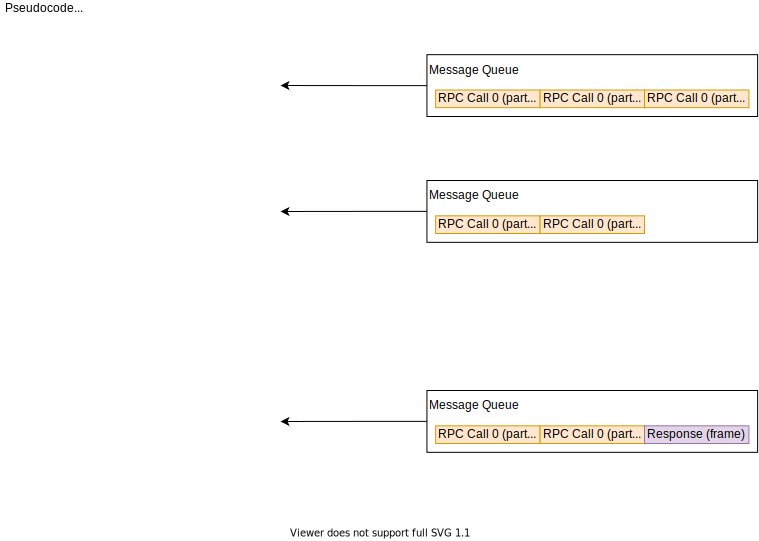
\includegraphics{./bugs/memoryreq.pdf}
        }
    % \vspace{-1in}
    % \caption{Example bug encountered during for our RPC implementation}
    % \label{fig:bug_mm_req}
    
\end{figure}
